\documentclass{sigchi}

% Use this command to override the default ACM copyright statement (e.g. for preprints). 
% Consult the conference website for the camera-ready copyright statement.
\toappear{
  Submitted for review.
}

% Arabic page numbers for submission. 
% Remove this line to eliminate page numbers for the camera ready copy
\pagenumbering{arabic}


% Load basic packages
\usepackage{balance}  % to better equalize the last page
\usepackage{graphicx} % for EPS, load graphicx instead
\usepackage{times}    % comment if you want LaTeX's default font
\usepackage{url}      % llt: nicely formatted URLs
\usepackage{subfigure}
\usepackage{tikz}

%\linespread{2}

% llt: Define a global style for URLs, rather that the default one
\makeatletter
\def\url@leostyle{%
  \@ifundefined{selectfont}{\def\UrlFont{\sf}}{\def\UrlFont{\small\bf\ttfamily}}}
\makeatother
\urlstyle{leo}


% To make various LaTeX processors do the right thing with page size.
\def\pprw{8.5in}
\def\pprh{11in}
\special{papersize=\pprw,\pprh}
\setlength{\paperwidth}{\pprw}
\setlength{\paperheight}{\pprh}
\setlength{\pdfpagewidth}{\pprw}
\setlength{\pdfpageheight}{\pprh}

% Make sure hyperref comes last of your loaded packages, 
% to give it a fighting chance of not being over-written, 
% since its job is to redefine many LaTeX commands.
\usepackage[pdftex]{hyperref}
\hypersetup{
pdftitle={SIGCHI Conference Proceedings Format},
pdfauthor={LaTeX},
pdfkeywords={SIGCHI, proceedings, archival format},
bookmarksnumbered,
pdfstartview={FitH},
colorlinks,
citecolor=black,
filecolor=black,
linkcolor=black,
urlcolor=black,
breaklinks=true,
}

% create a shortcut to typeset table headings
\newcommand\tabhead[1]{\small\textbf{#1}}


% End of preamble. Here it comes the document.
\begin{document}

\title{Gesture Beyond the Surface: Online Continuous Gesture Recognition}

\numberofauthors{2}
\author{
  \alignauthor 1st Author Name\\
    \affaddr{Affiliation}\\
    \affaddr{Address}\\
    \email{e-mail address}\\
  \alignauthor 2nd Author Name\\
    \affaddr{Affiliation}\\
    \affaddr{Address}\\
    \email{e-mail address}\\
}

\maketitle

\begin{abstract}
under challenging conditions with different lighting conditions
\end{abstract}

\keywords{
  Guides; instructions; author's kit; conference publications;
  keywords should be separated by a semi-colon.
}

\category{H.5.m.}{Information Interfaces and Presentation (e.g. HCI)}{Miscellaneous}

\section{Introduction}

% Abstract Hidden Markov Model for online continuous gesture recognition with
% unbounded and unsegmented RGB and depth video sequences. 

\section{Related Work}
Bag-of-feature approach is similar to the bag-of-word approach in document classification.
To represent an image using BoW model, an image can be treated as a document. Similarly,
``words'' in images need to be identified too. To achieve this, it usually includes
following three steps: feature detection, feature description and code book generation~\cite{fei2005}.
In the bag-of-word approach for document classification, the notion of order of words is lost
~\cite{Russell2003}. Higher-order $n$-gram models maintain some local notion of word order.

Heng et al. did an evaluation of several feature detectors and descriptors for action
recognition in video sequences~\cite{wang2009}. They used the same bag-of-features SVM classification
method for all the feature detector and descriptor combinations.
Codebook With the bag of words

SVM does not usually handle time series data. To use SVM for time series, one
can concatenate the input in a time series into one long vector sample. scale
short time
action recognition

Advantages of HMM
~\cite{sharma00, Starner95}
\begin{itemize}
  \item Can specify more constraints in the the parameters, i.e. use Bakis model. to reduce the total number of parameters
It is harder to impose Bakis model to HHMM since the hidden states are shared. The state transition probability for $S_t$ in HHMM
is $|S|^2 \times |G| $. In mixture HMMs model, it is $k\times |S|\times|G|$ where $k$ is the number of states a state can transit to.
\end{itemize}

If we do not constrain the transition in the hidden states $S_t$, HHMM may have a fewer number of parameters because of the states sharing.
If we constrain the transition, specifying more structures in the sub HMMs, the mixture of HMMs can have fewer number of parameters.

Training HMMs separately and combining them into HHMM for gesture inference. No across-gesture sharing (of hidden states)

dynamic time warping

dense sampling cite
\subsection{Hand Tracking}
Marcos-Ramiro et al. ~\cite{marcos2013} develop a method of computing hand likelihood maps based on RGB videos. Optical flow
hands show more movement. Our method is very similar to their approach but we combine both RGB images and depth images to compute
the gesture salience map. They hypothesized that given a frontal, static camera pointing to the upper body of a person, hands are
normally the parts of the image that show more movement. The two strong indicators are:

Space-time interest point
\section{Implementation Details}
PCA reduction. The features are in the PC space, so they should have small correlations.
So we set the covariance matrices for the Gaussian CPD to be diagonal.


Local space-time features capture characteristic shape and motion in video and
provide relatively independent representation of events with respect to their
spatio-temporal shifts and scales. \cite{wang-spatio-2009}


\cite{wang-spatio-2009}

Kinect skeleton tracking methods random forest

\section{System Overview}
Our online continuous hand gesture recognition framework consists mainly two parts: feature
extraction and gesture classification.

\begin{figure*}
\centering
\includegraphics[width=1\linewidth, trim=0mm 10mm 0mm 10mm,
clip]{figure/system.ps}
\caption{}
\label{fig:feature}
\end{figure*}

Feature extraction on video sequences can be broken down into two steps: 1)
detect points of interest by maximizing certain salience functions; 2) compute
feature descriptors to capture shape and motion in the neighborhoods of selected
points~\cite{wang-spatio-2009}.

For hand gesture recognition, the points of interest are certainly the hands. While the skeleton tracking provided
by the Kinect SDK is quite robust most of the time, its error for the hand joint tracking increases when
the hands are close to the body or move quickly (see Figure~\ref{fig:compare-skeleton}). As a result, we
develop the gesture salience detection method to locate the gesturing hand more accurately.
 
\section{Gesture Salience Detection}

Similar to Marcos-Ramiro et al.~\cite{marcos2013}, we define gesture salience as a function of 
the closeness of the motion to the observer (e.g., the camera) and the magnitude of the motion.

For a given data frame from the RGB-D camera, we combine both the RGB and the depth data to 
compute gesture salience. Both the RGB and the depth data can be noisy. RGB cameras are sensitive to lighting conditions (cite).
Skin color based detection can be sensitive to the clothes users wear. Depth cameras based on 
structured light sensors, such as the first generation Kinect sensor, compare the projected infra-red pattern
with the reflected one to determine depth~\cite{welsh:2011}. As a result, they do not work well on 
objects that are highly reflective (mirrors and shiny metal) or highly absorptive (fluffy and/or dark materials such as human hair)
\footnote{\url{http://msdn.microsoft.com/en-us/library/hh855356.aspx}}. By combining the two,
the overall gesture salience detection can be more robust to noise.

The following are the detailed steps of our gesture salience detection method for each frame. 
We show the illustrations in Figure~\ref{fig:gesture-salience}. 

\subsection{Skin Segmentation}
We use an off-the-shelf simple skin color detection method which is not trained on our data set to do a binary segmentation. The reason is
to make the method generalizable to any users and environment. We compute a binary skin mask, $M^S$, based on the RGB image converted into YCrCb
color space.  We also find the user mask, $M^U$ obtained from the Kinect SDK based on the depth image. 
We then align $M^S$ with $M^U$ and find their intersection $M^{S\wedge U}$, which indicates the skin region on the user.

\subsection{Motion Detection}
Similar to Cutler and Turk~\cite{cutler1998}, we compute the motion mask for the current depth frame based on 3 frames. We first filter each 
depth frame by the user and skin mask $M^{S\wedge U}$ at time $t$, and then
smooth it through a median filter to obtain $D_t$  (Figure~\ref{fig:skin-mask}).
Equation~(\ref{eq:motion-mask}) computes the binary mask, $M_{t\vee t-1}^M$, indicating moved pixels at either time $t$ or $t - 1$ (Figure~\ref{fig:motion-mask}).
$D_{t\vee t-1}^{D}$ is the absolute difference between $D_t$ and $D_{t-1}$, and $T$ is the threshold operator that filters out small change in depth value 
(we set the threshold to be 15mm). 
To obtain the motion mask, $M_{t}^M$ for time $t$ only, we use $M_{t-1\vee t-2}^M$, the motion mask for $t-1$ and $t-2$ as well (see Equation~(\ref{eq:motion-mask-t-1})-(\ref{eq:motion-mask-t}),
symbols $\wedge$ and $\oplus$ are the AND and XOR operators respectively).
\begin{align}
M_{t\vee t-1}^M &= T(D_{t\vee t-1}^{D}) \label{eq:motion-mask} \\
M_{t-1}^M &= M_{t\vee t-1}^M \wedge M_{t-1\vee t-2}^M \label{eq:motion-mask-t-1}\\
M_{t}^M &= M_{t\vee t-1}^M \oplus M_{t-1}^M \label{eq:motion-mask-t}
\end{align}

\subsection{Salience Map}
We apply histogram equalization to both $D_t$ and $D_{t\vee t-1}^{D}$ to obtain cumulative distributions $H_t$ and $H_{t\vee t-1}^D$.
$H_t$ represents the probability of salience given a depth value and $H_{t\vee t-1}^D$ represents the probability of salience given
a depth difference value. The lower the depth value or the higher the depth difference value, the higher the salience probability.
Finally the salience map (Figure~\ref{fig:salience}) can by computed for each pixel $(x, y)$ as
\begin{align}
S_t(x, y) = H_t(D_t(x, y)) \times H_{t\vee t-1}^D(D_t^D(x, y)) \times M_t^M
\end{align}
The multiplication of the binary motion mask $M_t^M$ allows us to only consider the motion due to the user at $t$.
 
\subsection{Salience Location}
The final step of locating the most salient region in a frame is finding the
contour, $C_t$, from the salience map $S_t$ that has a perimeter greater than
the smallest possible hand perimeter and with the highest average salience for all the pixels in side the contour.

When motion is slow, the motion mask usually indicates the edge of the moving
object. As a result, the center of $C_t$ may not be the center of the moving
object (in our case, the user's hand). Hence, we use 2 iterations of Camshift~\cite{Bradski98} on the depth image $D_t$ with a start search location at then center of $C_t$ to refine
the final bounding box, $B_t$, of gesture salience (Figure~\ref{fig:camshift}).

\begin{figure*}[tb]
\centering
\hspace{-0.6em}%
\subfigure[]{
\includegraphics[width=0.195\linewidth]{figure/color.eps}\hspace{-0.6em}%
\label{fig:color}
}
\subfigure[]{
\includegraphics[width=0.195\linewidth]{figure/depth.eps}\hspace{-0.6em}
\label{fig:skin-mask}
}
\subfigure[]{
\includegraphics[width=0.195\linewidth]{figure/motion-mask1.eps}\hspace{-0.6em}
\label{fig:motion-mask}
}
\subfigure[]{
\includegraphics[width=0.195\linewidth]{figure/salient-map.eps}\hspace{-0.6em}
\label{fig:salience}
}
\subfigure[]{
\includegraphics[width=0.198\linewidth]{figure/bounding-box.eps}
\label{fig:camshift}
}
\caption{Gesture salience detection steps: \subref{fig:color} RGB image under low lighting condition;
\subref{fig:skin-mask} depth map $D_t$ filtered by skin and user mask, $M^{S\wedge U}$. False detection of skin due to
clothes color similar to skin color; \subref{fig:motion-mask} motion mask,  $M_{t\vee t-1}^M$, indicating moved pixels for time $t$ and $t-1$;
\subref{fig:salience} salience map with red color indicating high probability of the salience; 
\subref{fig:camshift} final gesture salience bounding box, $B$. (Best viewed in
color.)}
\label{fig:gesture-salience}
\end{figure*}

Figure~\ref{fig:compare-skeleton} compares the results of gesture salience detection for hand gestures with the skeleton tracking results
from the Kinect SDK.
\begin{figure*}
\centering
\subfigure[]{
\includegraphics[width=0.24\linewidth]{figure/rotate-color.eps} \hspace{-0.6em}
}
\subfigure[]{
\includegraphics[width=0.24\linewidth]{figure/rotate-depth.eps} \hspace{-0.6em}
}
\subfigure[]{
\includegraphics[width=0.24\linewidth]{figure/near-body-color.eps}
\hspace{-0.6em} }
\subfigure[]{
\includegraphics[width=0.24\linewidth]{figure/near-body-depth.eps}
\hspace{-0.6em} }
\caption{Comparison between gesture salience detection for hand gestures and skeleton tracking from the Kinect SDK. The green lines are
the skeleton tracking results. The red region is the detected salient gesture
region using our method. (Best viewed in color.)}
\label{fig:compare-skeleton}
\end{figure*}

\section{Online Continuous Gesture Recognition}
\subsection{Feature Descriptor}
From the bounding box, $B_t$, of the detected gesture salience, we compute both
motion trajectory feature $X_t^M$ and hand pose feature $X_t^P$. 

The motion trajectory feature $X_t^M$ include relative
position from $B_t$ to the center of the shoulders
($\mathbf{p}$), velocity ($\mathbf{v}$), and acceleration ($\mathbf{a}$). The position of the shoulder center from the Kinect
skeleton tracking is relatively accurate all the time. The 3-dimensional
vectors $\mathbf{p}$, $\mathbf{v}$, $\mathbf{a}$ are in the world coordinate systems.

For hand pose features, we extract a $64\times 64$ px
image patch, $I_t$, with depth-mapped values from $B_t$.
We denoise, $I_t$, using a morphological close operation and then compute the
HOG feature descriptor~\cite{dalal05}, $I_t^H$, from it. The cell size we use is
$4\times 4$ px and the number of orientation bins is 9. Our earlier work (under
submission) shows that finer grained HOG descriptor for hand poses gives better
recognition accuracy. We also only use one fold of normalization because depth
values are less affected by illumination variation and contrast normalization is
not necessary. This results in a $14\times 14\times 9$ length $I_t^H$.

Similar to Wang et al.~\cite{wang-spatio-2009}, we apply dimension reduction on
$I_t^H$ concatenated as a column vector using principal component analysis on
training data.
The final hand pose feature $X_t^P$ is obtained by projecting $I_t^H$ to a lower
dimensional space with dimension $k$.

The final feature vector $X_t$ combined from $X_t^M$ and $X_t^P$ has dimension
$9 + k$. They are standardized to have zero mean and unit variance.
Figure~\ref{fig:feature} shows a visualization of the feature vectors with $k=7$
for a sequence of continuous gestures with rest poses in between. The regions of
smoothness indicate rest poses while the regions of rapid changes indicate
gestures.

\begin{figure}
\centering
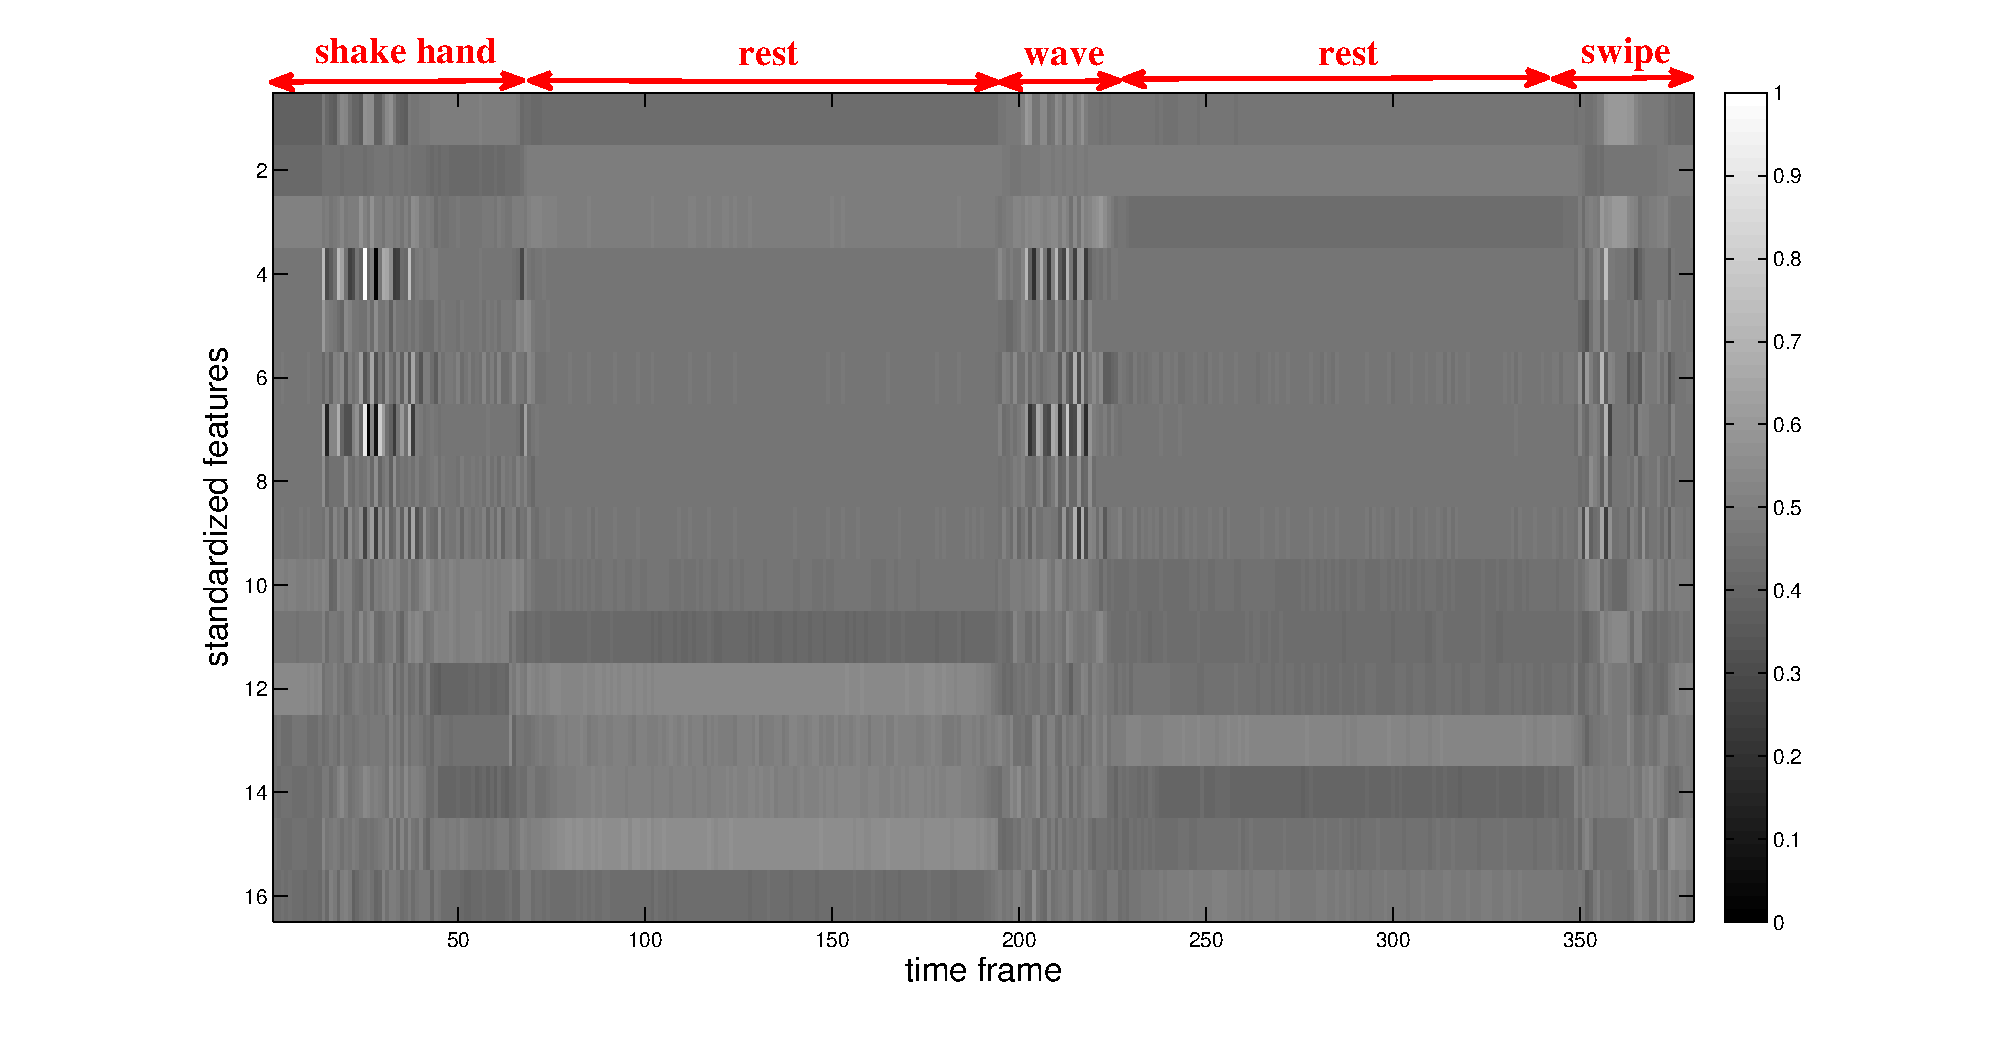
\includegraphics[width=1\columnwidth,trim=20mm 5mm 30mm 1mm,
clip]{figure/pca16.eps}
\caption{}
\label{fig:feature}
\end{figure}

\subsection{Training AHMM for Gesture Recognition}
Our earlier work (under submission) has shown that the 1-level abstract hidden
Markov model (AHMM) closely models the gesture production process and
incorporates gesture recognition and gesture segmentation at the same time. In
this work we give a quantitative comparison between a model trained from AHMM
and one trained from a mixture of HMMs. (cite)

Figure~\cite{fig:ahmm} shows the model represented in a dynamic Bayesian network
(DBN). It is closely related to the hierarchical hidden Markov
model~\cite{murphy02}. Node $G_t$ represents the gesture that the
user is making at time $t$. It includes different gesture phases the system
can recognize.
Node $S_t$ is the hidden state of the hand movement, which is essentially a
vector quantization of the actual, observed (but noisy) feature vector $X_t$. 
Node $F_t^G$ is a binary variable that indicates the end of a
gesture. It is ``on'' (has value 1) if the lower level HMM at time $t$ has just
``finished'', otherwise it is ``off'' (value 0). $G_{t+1}$ can only change value
from $G_t$ if $F_t^G$ is ``on''. Note that $G_t$, $S_t$, and $F_t^G$ take
discrete values, so the conditional probability distributions (CPDs) for them
can take a tabular form. $X_t$ is a vector with continuous values and we use a
Gaussian distribution for its CPD, i.e.,
\begin{align}
P(X_t = x_t | S_t = i) = N(x_t; \mu_i, \Sigma_i)
\end{align}

\begin{figure}
\centering
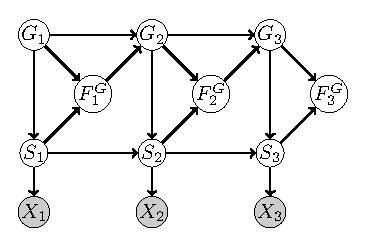
\includegraphics[]{figure/ahmm.eps}
\caption{Gray color indicates observed nodes.}
\label{fig:ahmm}
\end{figure}

During the training process, we give the model sequences of difference gestures
with labeled $G_t$ and $F_t^G$ that correspond to the observed feature vectors
$X_t$, but $S_t$ is hidden. There can be different gestures in one sequence. In
this way, the model can learn the termination probability given a hidden state
and a gesture phase, i.e.,
$P(F_t^G = 1 | G_t = g, S_t = i)$, and the transition probability between two
hidden states given the gesture phase, i.e., $P(S_t = j | G_{t - 1} = g,
S_{t - 1} = i)$. Note that the transition probabilities learned are for both
within a gesture and between gestures.

Compare this with the mixture HMMs previously used for gesture recognition,
AHMM allows sharing of substructures (i.e., hidden states $S_t$) across
different gestures and thus reduces the total number of hidden states. It is
also easier to learn the transition probabilities between hidden states across
gestures in AHMM than in the mixture of HMMs~\cite{murphy02}.

\tikzstyle{vertex}=[circle, draw, minimum size=16pt, inner sep=0pt]
\tikzstyle{observed-vertex}=[circle, draw, minimum size=16pt, inner
sep=0pt, fill=black!20] 
\tikzstyle{edge} = [draw, thick, -]
\tikzstyle{directed-edge} = [draw, thick, ->]

\begin{figure}[tb]
\centering
  \begin{tikzpicture}[auto,swap, scale=1.5]
    % First we draw the vertices
    \foreach \pos/\name in {{(1, 2)/G_1}, {(4,2)/G_2},
      {(0, 1)/S_{11}}, {(1, 1)/S_{12}}, {(2, 1)/S_{13}}, {(3, 1)/S_{21}}, {(4,
      1)/S_{22}}, {(5, 1)/S_{23}}} 
    \node[vertex] (\name) at \pos {$\name$};
    \foreach \pos/\name in {{(0, 0)/X_{11}}, {(1, 0)/X_{12}}, {(2, 0)/X_{13}},
    {(3, 0)/X_{21}}, {(4, 0)/X_{22}}, {(5, 0)/X_{23}}}
      \node[observed-vertex] (\name) at \pos {$\name$};
    % Connect vertices with edges and draw weights
    \foreach \source/ \dest in {G_1/S_{11}, G_1/S_{12}, G_1/S_{13},
    S_{11}/X_{11}, G_2/S_{21}, G_2/S_{22}, G_2/S_{23}, S_{12}/X_{12},
    S_{13}/X_{13}, S_{21}/X_{21}, S_{22}/X_{22}, S_{23}/X_{23}, S_{11}/S_{12}, S_{12}/S_{13},
    S_{21}/S_{22}, S_{22}/S_{23}} \path[directed-edge] (\source) -- (\dest);
  \end{tikzpicture}
  \caption{A mixture of HMMs~\cite{murphy02}.}
  \label{fig:amms}
\end{figure}

Since $S_t$ is hidden, we use expectation maximization (EM)
algorithms to learn the maximum likelihood estimate of the model parameters for
all the CPDs. The performance of EM can be highly dependent on how the algorithm
is initialized~\cite{dicintio2012} and it tends to converge to a local maximum
of the observed data likelihood. As we model the $P(X_t | S_t)$ as a Gaussian
distribution, we can view $X_t$ as a mixture of Gaussians. The number of states 
$S_t$ can take is the number of mixtures (i.e., clusters). As a result, we
perform an unsupervised clustering analysis on a sub-sample of training data and
use the Bayesian information criterion (BIC)~\cite{fraley12} to find the optimal
number of clusters.

Then we set the number of state for $S_t$
to be the number of clusters, and initialize $\mu_i$ to be the cluster centers.
We have tested with different clustering methods, including $k$-means,
and mixture of Gaussians with $k$-means initialization, multiple random
initializations, or hierarchical clustering initialization~\cite{Fraley:2003}. We
found that the hierarchical clustering initialization used in the \texttt{mclust} package in R
language gives the best final recognition accuracy result.

\subsection{Online Recognition}
Difference inference methods exist for DBNs, exact or approximate, offline or
online, with accuracy and speed trade-offs. As a first step, we use the
2TBN-based (2-slice temporal Bayes net) junction tree algorithm as the lower
level 
engine~\footnote{\url{http://bnt.googlecode.com/svn/trunk/docs/usage_dbn.html}}
to do exact inference on the graph. During the training process, we combine it
with the offline forwards-backwards message passing operators to smooth the
estimation using the entire evidence sequence.

During the online recognition process, we use the ``fixed-lag-smoothing''
method~\cite{murphy02} to allow a few frames lag in order to use more evidence to smooth the recognition result. This means, at time $t$,  we estimate the most likely
gesture at $t - L$ as:
\begin{align}
g* = \arg\max_g P(G_{t-L} = g | x_{1:t})
\end{align}
where $L$ is the lag time. At each time frame $t$, we compute the forward
message $\alpha_t(i)$ from $\alpha_{t-1}(i)$. Then we do a backward message pass
until $t-L$ to estimate the gesture phase at $t - L$.

\section{Experimental Evaluation}
Using a public gesture corpus
ChAirGest\cite{Ruffieux2013}, 
we conduct user-dependent evaluation 
feature detection methods

\subsection{Data Set}
We use part of the ChAirGest corpus as our data set. We include data from
both lighting conditions: normal and low intensity. However we do not use the
data from the Xsens which are inertial measurement unit (IMU) sensors because we
think it is not likely that users would wear them in a realistic setting. We
only use the RGB, depth and skeleton stream data from the Kinect which is less
obtrusive.

There are 10 gestures (swipe left (\#1), swipe right (\#2), push to screen
(\#3), take from screen (\#4), palm-up rotation (\#5), palm-down rotation (\#6),
draw a circle with rotating palm (\#7), draw a circle with palm down (\#8), wave
hell (\#9) and shake hand (\#10)) and 3 resting postures (hands on then table,
hands on the belly , and hands under the chin) in the corpus.
Each gesture consists consists labeled pre-stroke, gesture nucleus and
post-stroke~\cite{Pavlovic97} phases.

We use recordings from 8 participants (out of 10 because we have data
corruption problem with the rest 2), and for each participant, we use 2 sessions
of recordings.
In each session, there are 7-8 sequences with 2-5 gesture occurrences per
sequence. Overall there are 2 occurrence for each gesture/resting posture combination per subject.

\subsection{Method}
For each participant, we use
one tenth of the sequences for testing and the remaining for training. 
The RGB and depth videos are 30 fps (frame per second) and we down-sample them
to 10 fps to increase the training speed. This results in about 600 frames per sequence on average.

We treat the preparation phase (\#11), the retraction phase (\#12) and the rest posture (\#13) 
as different gesture classes, resulting
in 13 gesture classes. The a random guess accuracy would be
7.8\%.


In this data set, all gesture occurrences follow the pattern: rest $\rightarrow$ preparation
$\rightarrow$ gesture nucleus $\rightarrow$ retraction $\rightarrow$ rest and then repeat. 
Hence, we initialize the prior distribution CPD
and the transition probability CPD for $G$ such that the probability of transition from the preparation phase
to one of the ten gesture nucleus phases is uniform and all other transitions are deterministic.

We use features computed using our mehtod described in the earlier section based
on the training data from one participant to do mixture of Gaussian clustering analysis\footnote{\url{http://cran.r-project.org/web/packages/mclust/index.html}}. 
Our results show that $50$ clusters and
$11$ features give the highest BIC. Hence we set the 
number of hidden states $S_t$ to be $50$ and $k = 2$
in the PCA dimensionality reduction of the hand pose feature $X_t^P$.

To compare recognition performance, we compute per frame accuracy and F1 score. 
A frame is considered correctly classified if its predicted label is equal to the ground truth label.
Hence frame accuracy is computed as
\begin{displaymath}
\text{frame accuracy} = \frac{\text{\# correctly classified frames}}{\text{\# frames in the sequence}}
\end{displaymath}
Because we have a multi-class classification problem, we compute F1 score for each gesture class and 
the overall F1 score is the average from all gesture classes. All results
reported here are for the test data set.

\subsection{Comparison of Feature Detection Methods}
% \begin{table}
%   \centering
%   \begin{tabular}{|c|c|c|}
%     \hline
%     \tabhead{Objects} &
%     \multicolumn{1}{|p{0.3\columnwidth}|}{\centering\tabhead{Caption --- pre-2002}} &
%     \multicolumn{1}{|p{0.4\columnwidth}|}{\centering\tabhead{Caption --- 2003 and afterwards}} \\
%     \hline
%     Tables & Above & Below \\
%     \hline
%     Figures & Below & Below \\
%     \hline
%   \end{tabular}
%   \caption{Table captions should be placed below the table.}
%   \label{tab:table1}
% \end{table}
We compare our gesture salience feature detection method with 2 two other
methods based on their effect on the gesture recognition performance. 

\textbf{Dense} sampling is the simplest method which extracts features at
regular positions in a image. It was used in both action recognition~\cite{wang-spatio-2009}
and gesture recognition~\cite{konecny2012}.

Skin \& Kinect skeleton method finds the skin contour closest to the right hand
joint from the skeleton tracking result provided by Microsoft's Kinect SDK.

We use the same HOG feature descriptor with $4\times 4$ px cell sizes and 9
orientation bins, and reduces the feature dimension using PCA.
No motion trajectory features are used for dense sampling, whereas the
9-dimensional motion trajectory feature $X^M$ is included for both Skin \&
Kinect skeleton method and gesture salience method.
Table~\ref{tab:feature-detection} shows their performance on gesture recognition using the same AHMM training and offline smoothing during recognition.

\begin{table}
\centering
\begin{tabular}{|l|l|l|}
\hline
\tabhead{Feature detector} & {\tabhead{Accuracy (std.)}} & {\tabhead{F1 (std.)}}\\
\hline
Dense sampling upper body & 68.0\% (4) & 57.7\% (8)\\
\hline
Skin \& Kinect skeleton & 72.1\% (16) & 64.7\% (11) \\
\hline
Gesture salience & \textbf{76.7\%} (4) & \textbf{69.3\%} (6) \\
\hline
\end{tabular}
\caption{}
\label{tab:feature-detection}
\end{table}

The results show that our salience detection method give the best performance.
It is possible that dense sampling may work better for gestures with big arm
movement away from the body. However in our data set, there are gestures with
small movement and close to the body (e.g., swipe left/right, take from screen).

The lower performance using skin & Kinect skeleton method shows that error
in feature location detection (in this case due to error in skin detection and
skeleton tracking) will affect the recognition performance.


\subsection{Comparison of Feature Descriptor}
We also compare the recognition results without and with the hand pose feature
$X_t^P$. The results in Table~\ref{tab:hand-pose-feature} shows that the
performance are comparable with the results for using the hand pose feature very
slightly higher. This may be due to the fact that most of the gestures in the
data set are distinguishable based on motion trajectory. However, by comparing
Figure~\ref{fig:cm9} and \ref{fig:cm11}, we can see that the hand pose features
still help improve the recognition accuracy for certain gestures such as ``swipe right'' (\#2), ``push to screen'' (\#3), ``take from screen'' (\#4).
The ``take from screen'' has dynamic hand pose (grab motion) and hence, the hand
pose feature can provide additional information for its recognition.

We also not that the noise in the hand pose feature due to variations in
localizing the center of salience can also contribute to the decrease in
recognition accuracy for some gestures.

\begin{table}
\centering
\begin{tabular}{|l|l|l|}
\hline
\tabhead{Hand pose feature} & \tabhead{Accuracy (std.)} & \tabhead{F1 (std.)}\\
\hline
No hand pose feature & 76.5\% (5) & 68.4\% (7)\\
\hline
Use hand pose feature  & \textbf{76.7\%} (4) & \textbf{69.3\%} (6) \\
\hline
\end{tabular}
\caption{}
\label{tab:hand-pose-feature}
\end{table}

\begin{figure}
\centering
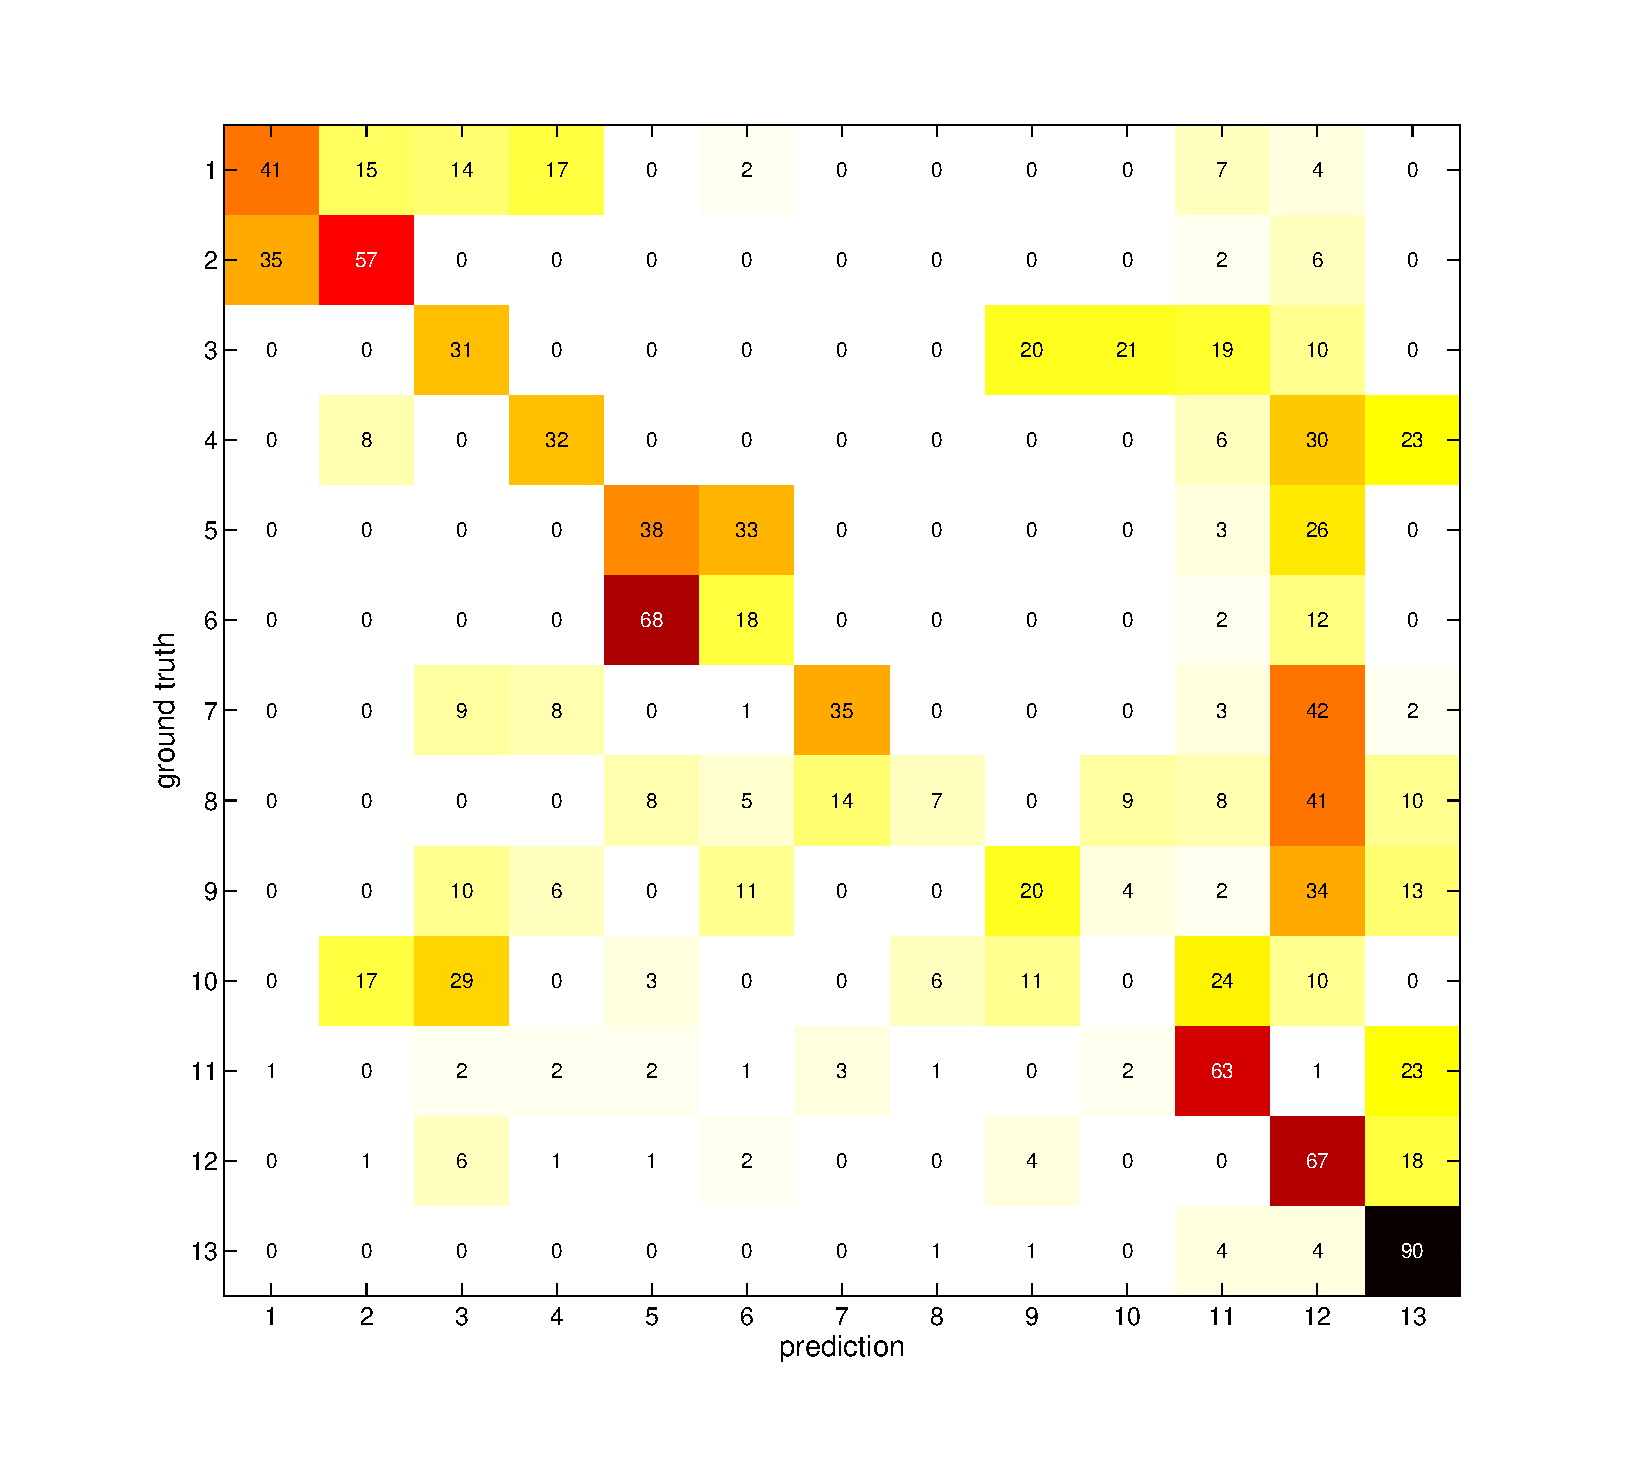
\includegraphics[width=1\columnwidth]{figure/cm9.eps}
\caption{Confusion matrix of ground truth gesture phase labels vs. predicted
gesture phase labels for frame when \textit{no hand pose features} are used.}
\label{fig:cm9}
\end{figure}

\begin{figure}
\centering
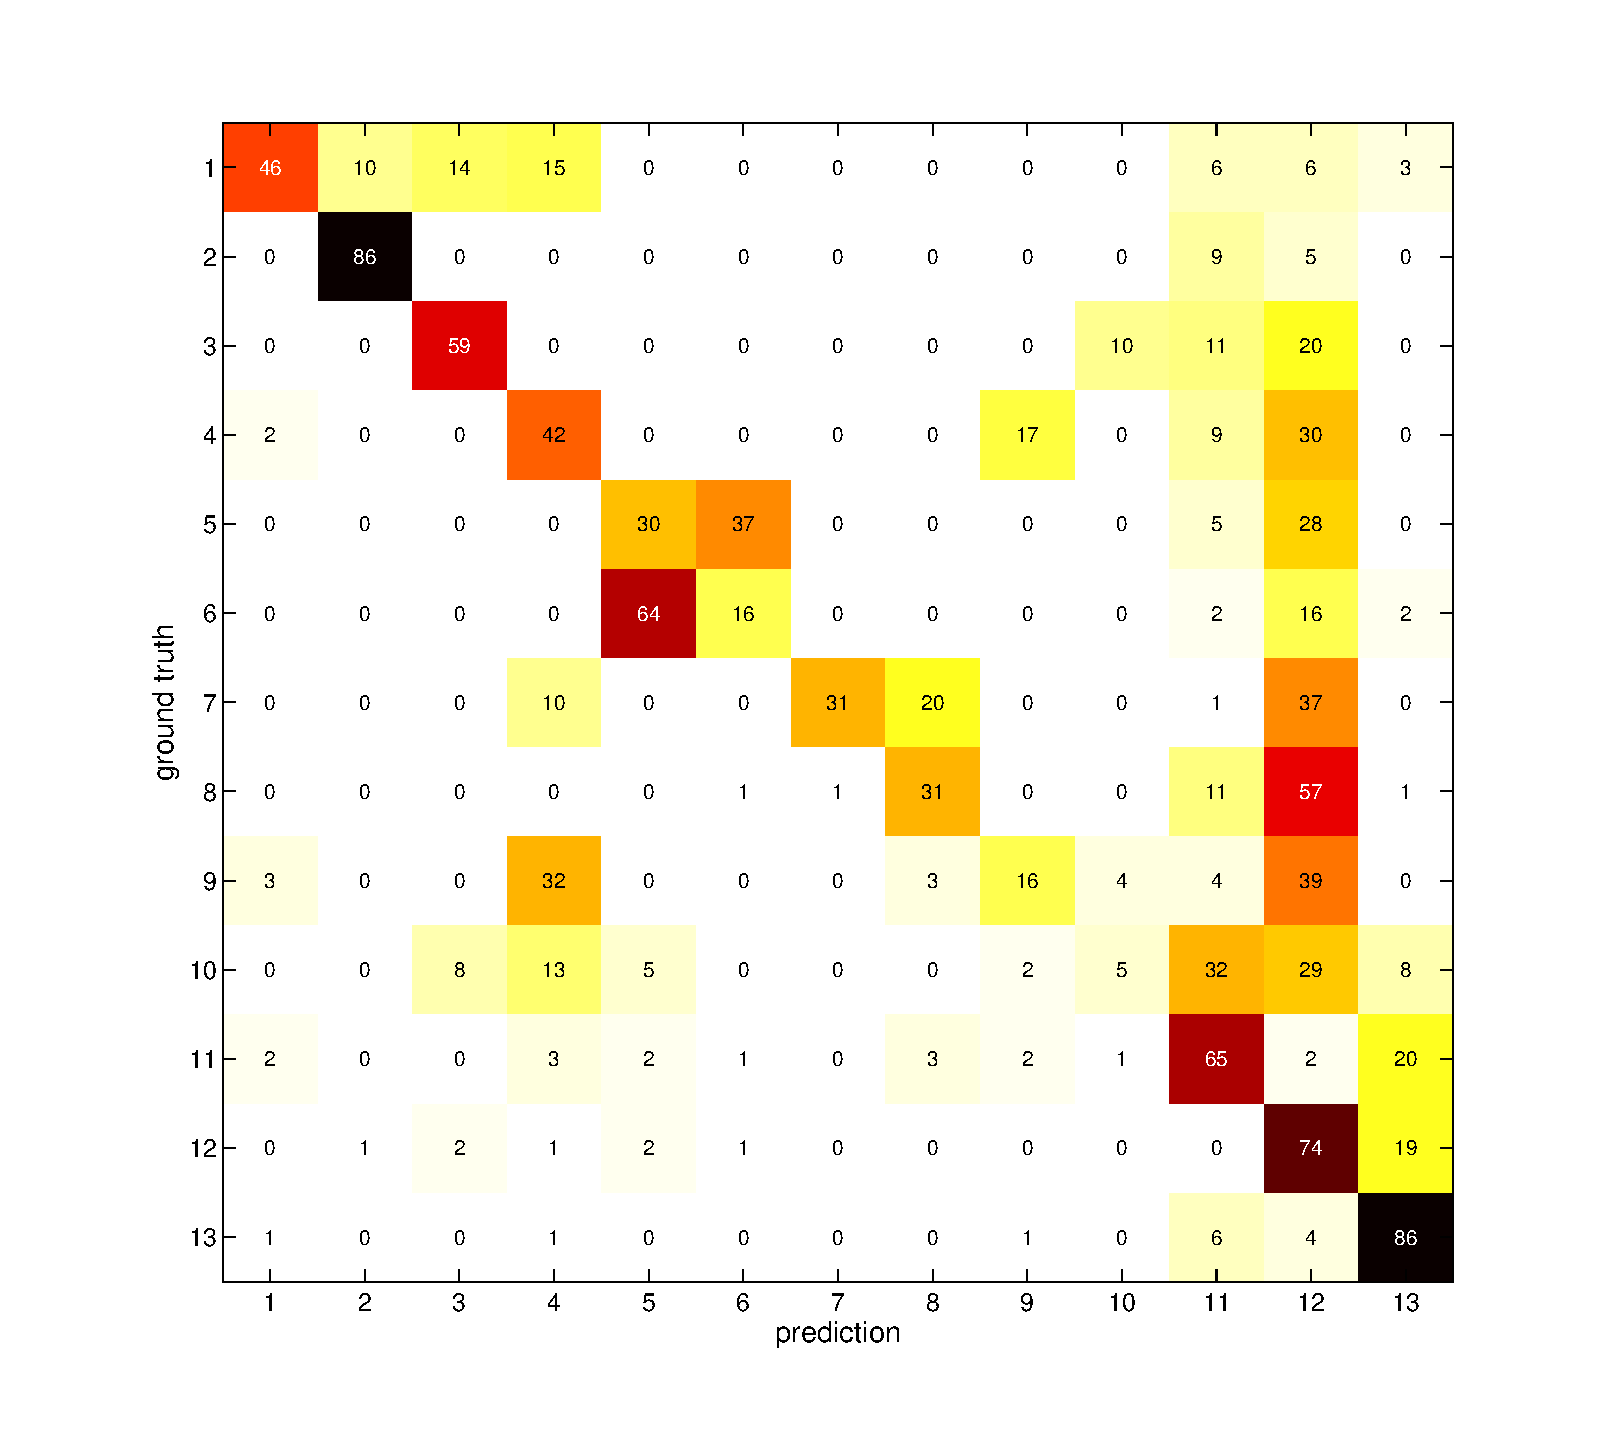
\includegraphics[width=1\columnwidth]{figure/cm11.eps}
\caption{Confusion matrix of ground truth gesture phase labels vs. predicted
gesture phase labels for frame when \textit{hand pose features} are used
($k=2$).}
\label{fig:cm11}
\end{figure}

\subsection{Comparison of Recognition Training Methods}
We give an qualitative comparison between the AHMM and the mixture HMMs for
gesture recognition in the earlier section. Hear we report our experiment
evaluation using two models to train the parameters. Same salience feature detector and descriptor
described in the earlier section are used for both training methods. Offline
smoothing is used for recognition for both. 

To train the mixture of HMMs, we segment the training sequences for each gesture
phase. For each gesture HMM, we use 5 hidden states and initialize the
transition probabilities uniformly. The means of the Gaussian distribution CPD
$P(X_t|S_gt)$ is initialized using mixture of Gaussians clustering as well. We
also learn the termination probability of each hidden state for gesture phase
$g$ as well.

As the mixture of HMMs do not handle termination and transition directly, we use
the learned parameters in a hierarchical HMM shown in
Figure~\ref{fig:ahmm-reset}. This model is similar to AHMM in
Figure~\ref{fig:ahmm} with one distinction: the hidden state $S_t$ resets if
then previous gesture terminates (represented by the directed edge from $F_t^G$
to $S_t$). In this case, the prior probability, i.e., $P(S_1 = j | G_1 = i)$
learning during mixture of HMMs can be used.

\begin{figure}
\centering
\includegraphics[]{figure/ahmm-reset.eps}
\caption{Gray color indicates observed nodes.}
\label{fig:ahmm-reset}
\end{figure}

The advantage of HMM training is that it reduces the total number of
state transition parameters to be learned and hence reduces the
complexity of the model. The inference algorithm on HMM can be faster than
the junction tree algorithm. However, the results in Table~\ref{tab:training}
show that the performance using mixture of HMMs training is much lower showing
that the state transition probabilities across the gestures can help imrove the
gesture recognition accuracy.

\begin{table}[t]
\centering
\begin{tabular}{|l|l|l|}
\hline
\tabhead{Training method} & {\tabhead{Accuracy (std.)}} & {\tabhead{F1 (std).}}\\
\hline
Mixture of HMMs & 50.6\% (17) & 55.6\% (8) \\
\hline
AHMM & \textbf{76.7\%} (4) & \textbf{69.3\%} (6) \\
\hline
\end{tabular}
\caption{}
\label{tab:training}
\end{table}

\subsection{Comparison of Online and Offline Inference}
Table~\ref{tab:inference} shows that our online inference method with 16
frames lag gives comparable results with offline inference. With 30fps data
stream, 16 frames is about half a second delay which might acceptable for human
reaction time.

\begin{table}[t]
\centering
\begin{tabular}{|l|l|l|}
\hline
\tabhead{Inference} & {\tabhead{Accuracy (std.)}} & {\tabhead{F1 (std).}}\\
\hline
Offline & 76.7\% (4) & 69.3\% (6) \\
\hline
Online (lag = 16 frames) & \textbf{76.9\%} (3) & \textbf{65.2\%} (9) \\ 
\hline
\end{tabular}
\caption{}
\label{tab:inference}
\end{table}


\section{Future Work}
Do away from skin color, what if the user wear glove, or like in the data set,
holding something in the hand. Better cleaning up of hand pose images.

\section{Conclusion}

% It is important that you write for the SIGCHI audience.  Please read
% previous years' Proceedings to understand the writing style and
% conventions that successful authors have used.  It is particularly
% important that you state clearly what you have done, not merely what
% you plan to do, and explain how your work is different from previously
% published work, i.e., what is the unique contribution that your work
% makes to the field?  Please consider what the reader will learn from
% your submission, and how they will find your work useful.  If you
% write with these questions in mind, your work is more likely to be
% successful, both in being accepted into the Conference, and in
% influencing the work of our field.

% Balancing columns in a ref list is a bit of a pain because you
% either use a hack like flushend or balance, or manually insert
% a column break.  http://www.tex.ac.uk/cgi-bin/texfaq2html?label=balance
% multicols doesn't work because we're already in two-column mode,
% and flushend isn't awesome, so I choose balance.  See this
% for more info: http://cs.brown.edu/system/software/latex/doc/balance.pdf
%
% Note that in a perfect world balance wants to be in the first
% column of the last page.
%
% If balance doesn't work for you, you can remove that and
% hard-code a column break into the bbl file right before you
% submit:
%
% http://stackoverflow.com/questions/2149854/how-to-manually-equalize-columns-
% in-an-ieee-paper-if-using-bibtex
%
% Or, just remove \balance and give up on balancing the last page.
%
\balance

% If you want to use smaller typesetting for the reference list,
% uncomment the following line:
% \small
\bibliographystyle{acm-sigchi}
\bibliography{gesture}
\end{document}
